\chapter{確率 - Probability}

\index{確率 - probability}

\key{確率 - probability}は0から1の間の実数で表されるある事象がどの程度の確率で起こりうるかを示すものです。
ある事象が確実に起こるなら確率は1であり、確実にあり得ないならその確率は0です。
ある事象の確率は$P(\cdots)$と表記され、3つの点がその事象を表します。

サイコロを投げるとき、その結果は1から6の整数で、それぞれの結果が 出る確率は1/6です。
このため、次のような確率が計算できる。

\begin{itemize}[noitemsep]
\item $P(\textrm{''4がでる''})=1/6$
\item $P(\textrm{''6以外''})=5/6$
\item $P(\textrm{''偶数''})=1/2$
\end{itemize}

\section{確率の計算 - Calculation}


ある確率を計算するには、組合せ論を用いるか、その事象が発生する過程をシミュレートする方法があります。
例えば、シャッフルした山札から同じ数字のカードを3枚引く確率を計算してみます。(例えば、$\spadesuit 8$, $\clubsuit 8$, $\diamondsuit 8$)。

\subsubsection*{方法1}

次の式を使うことができます。

\[\frac{\textrm{望ましい数量}}{\textrm{あり得る全体の数}}.\]

この問題では、各カードの価値は同じです。
このような結果は,$13 {4 \choose 3}$あります。
ある数を引く可能性は 13 パターンがあり、
その中で4つのスーツのうちから3つを引くのは
${4 \choose 3}$のパターンがあります。
ここで、全体の引くパターンは52枚のカードから3枚のカードを選ぶので、
${52 \choose 3}$です。
このため、この確率は以下の様になります。

\[\frac{13 {4 \choose 3}}{{52 \choose 3}} = \frac{1}{425}.\]

\subsubsection*{方法2}

今度はプロセスをシミュレ ーションするアプローチを考えます。
この例では、3枚のカードを引くので、3回のプロセスを実行します。
まず、1枚目のカードは何を選んでも良いです。
第2段階は, 51枚のカードが残っていて,そのうち3枚が最初のカードと同じ数なので$3/51$の確率で成功です。
同様に,3番目のステップも$2/50$の確率で 成功です。つまり、全体の処理が成功する確率は以下の様になります。

\[1 \cdot \frac{3}{51} \cdot \frac{2}{50} = \frac{1}{425}.\]

\section{事象 - Events}

確率における事象は集合として表現できます。
\[A \subset X\]
$X$はすべての可能な結果全体で、$A$は結果の部分集合です。
例えば、サイコロを振るとその結果は
\[X = \{1,2,3,4,5,6\}\]
となり、''偶数である''という集合は以下の通りです。
\[A = \{2,4,6\}\]

ある事象$x$には確率$p(x)$が割り当てられています。
そして、ある事象Aの確率P(A)は、次ように結果の確率の総和として計算することができます。
\[P(A) = \sum_{x \in A} p(x).\]
例えば、サイコロを投げる場合、各結果$x$に対して$p(x)=1/6$であるから、
''偶数である''という事象の確率は以下の通りです。
\[p(2)+p(4)+p(6)=1/2.\]

$X$ の確率は 1、つまり$P(X )=1$ です。
各事象は集合なので、標準的な集合演算で操作できます。

\begin{itemize}
\item \key{補集合 - complement} $\bar A$ は
''$A$ が起こらない''という意味です。
例えばサイコロにおいて、$A=\{2,4,6\}$の補集合は
$\bar A = \{1,3,5\}$です。
\item \key{集合和 - union} $A \cup B$ は
''$A$ か $B$ が起きる''という意味です。
$A=\{2,5\}$と$B=\{4,5,6\}$の和は、
$A \cup B = \{2,4,5,6\}$です。
\item The \key{集合積 - intersection} $A \cap B$は
''$A$ と $B$ が起きる''という意味です。
$A=\{2,5\}$ と $B=\{4,5,6\}$の集合積は
$A \cap B = \{5\}$です。
\end{itemize}

\subsubsection{補集合 - Complement}

補集合$\bar A$は次の様に計算できます。
\[P(\bar A)=1-P(A).\]

補集合を使うと、ある問題の逆を解くことで簡単に解けることがあります。
たとえば、サイコロを10回投げたとき、少なくとも1回6が出る確率は次の様に簡単に求められます。
\[1-(5/6)^{10}.\]

ここで、$5/6$は一投の結果が$6$でない確率です。
このため、$(5/6)^{10}$は10投のうちただの一回も1投も6でない確率である。これの補数が問題の答えとなります。

\subsubsection{集合和}

$A \cup B$の確率は以下の様に示ます。
\[P(A \cup B)=P(A)+P(B)-P(A \cap B).\]
例えば、サイコロを考えて、
\[A=\textrm{''偶数である''}\]
と
\[B=\textrm{''4未満である''}\]
であるとき、
\[A \cup B=\textrm{''偶数であるか4未満である''},\]
という確率は、
\[P(A \cup B) = P(A)+P(B)-P(A \cap B)=1/2+1/2-1/6=5/6.\]

事象$A$と$B$が\key{不連続,排他的 - disjoint}、すなわち$A \cap B$ が空である場合は事象$A \cup B$の確率は、単純に以下の様に示ます。

\[P(A \cup B)=P(A)+P(B).\]


\subsubsection{条件付き確率 - Conditional probability}

\index{条件付き確率 - conditional probability}

\key{条件付き確率 - conditional probability}
\[P(A | B) = \frac{P(A \cap B)}{P(B)}\]
というのは$B$が起こったと仮定した場合の$A$の確率である。
したがって、$A$の確率を計算するときは、$B$に属する結果だけを考えます。
先ほどのセットを使うと、
\[P(A | B)= 1/3,\]
となります。Bの結果は$\{1,2,3\}$で、そのうちの1つは偶数だからです。
つまり、結果が$1 \ldots 3$となった場合の偶数の結果の確率です。

\subsubsection{共通部分 - Intersection}

\index{独立 - independence}

条件付き確率を用いると共通部分である
$A \cap B$の確率は以下の様に求めることができます。
\[P(A \cap B)=P(A)P(B|A).\]
$A$と$B$が\key{独立 - independent}なのは次のときです。
\[P(A|B)=P(A) \hspace{10px}\textrm{and}\hspace{10px} P(B|A)=P(B),\]

ということは、$B$が起こっても$A$の確率は変わらず、その逆も同様ということです。
さて、この場合、共通部分の確率は
\[P(A \cap B)=P(A)P(B).\]
例えば、山札からトランプを引く場合、
\[A = \textrm{''the suit is clubs''}\]
\[B = \textrm{''the value is four''}\]
は独立です。このため、
\[A \cap B = \textrm{''クラブの4である''}\]
という確率は次の様に示ます。
\[P(A \cap B)=P(A)P(B)=1/4 \cdot 1/13 = 1/52.\]

\section{確率変数 - Random variables}

\index{確率変数 - random variable}

\key{ランダムな値 - random variable} はランダムに生成される値のことです。
例えば、2回サイコロを投げるとき、考えられる確率変数は
\[X=\textrm{''出た目の和''}.\]

例えば、結果が$[4, 6]$(最初に4で次に6だったという意味)であれば、$X$ の値は10とします。

例えば、2つのサイコロを投げるとき、$P(X=10)=3/36$です。
結果の総数は36であり、合計10を得るには、$[4,6]$, $[5,5]$, $[6,4]$ という3通りの可能性があるからです。

\subsubsection{期待値 - Expected value}

\index{期待値 - expected value}

\key{期待値 - expected value} $E[X]$ 確率変数 $X$ の平均値を示します。期待値は,以下の和として計算できます。
\[\sum_x P(X=x)x,\]
$x$は$X$でありうる全ての数です。

例えばサイコロを投げるとき、期待値は以下の通りです。
\[1/6 \cdot 1 + 1/6 \cdot 2 + 1/6 \cdot 3 + 1/6 \cdot 4 + 1/6 \cdot 5 + 1/6 \cdot 6 = 7/2.\]

期待値の面白い性質は\key{線形性 - linearity}です。
$E[X_1+X_2+\cdots+X_n]$
は常に
$E[X_1]+E[X_2]+\cdots+E[X_n]$.
と等しいです。
この式は、確率変数が互いに依存しあっていても成り立ちます。

例えば、2つのサイコロを投げるとき、期待される和は以下の通りです。
\[E[X_1+X_2]=E[X_1]+E[X_2]=7/2+7/2=7.\]

ここで、$n$個のボールが$n$個の箱にランダムに入れられ、
空箱の期待個数を計算する問題を考えます。
各球は等しい確率でどの箱にも入ります。$n = 2$の場合,次の様に考えられます。
\begin{center}
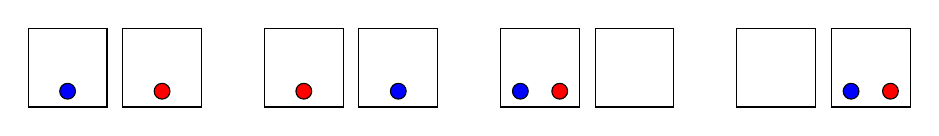
\begin{tikzpicture}
\draw (0,0) rectangle (1,1);
\draw (1.2,0) rectangle (2.2,1);
\draw (3,0) rectangle (4,1);
\draw (4.2,0) rectangle (5.2,1);
\draw (6,0) rectangle (7,1);
\draw (7.2,0) rectangle (8.2,1);
\draw (9,0) rectangle (10,1);
\draw (10.2,0) rectangle (11.2,1);

\draw[fill=blue] (0.5,0.2) circle (0.1);
\draw[fill=red] (1.7,0.2) circle (0.1);
\draw[fill=red] (3.5,0.2) circle (0.1);
\draw[fill=blue] (4.7,0.2) circle (0.1);
\draw[fill=blue] (6.25,0.2) circle (0.1);
\draw[fill=red] (6.75,0.2) circle (0.1);
\draw[fill=blue] (10.45,0.2) circle (0.1);
\draw[fill=red] (10.95,0.2) circle (0.1);
\end{tikzpicture}
\end{center}
このとき、空の箱の数は以下の通りです。
\[\frac{0+0+1+1}{4} = \frac{1}{2}.\]
一般に1つの箱が空の確率は、
\[\Big(\frac{n-1}{n}\Big)^n,\]
で求められます。その箱にボールが入っていないからです。
ここで線形性を利用すると期待値は次の様になります。
\[n \cdot \Big(\frac{n-1}{n}\Big)^n.\]

\subsubsection{分布 - Distributions}

\index{分布 - distribution}

\key{分布 - distribution}とは$X$が持ちうる各値の確率を示します。
分布は、値 $P(X=x)$ から構成されます。
2つのサイコロを投げるとき、その和の分布は次のようになります。

\begin{center}
\small {
\begin{tabular}{r|rrrrrrrrrrrrr}
$x$ & 2 & 3 & 4 & 5 & 6 & 7 & 8 & 9 & 10 & 11 & 12 \\
$P(X=x)$ & $1/36$ & $2/36$ & $3/36$ & $4/36$ & $5/36$ & $6/36$ & $5/36$ & $4/36$ & $3/36$ & $2/36$ & $1/36$ \\
\end{tabular}
}
\end{center}

\index{一様分布 - uniform distribution}
\key{一様分布 - uniform distribution},
the random variable $X$ has $n$ possible
values $a,a+1,\ldots,b$ and the probability of each value is $1/n$.
For example, when throwing a dice,
$a=1$, $b=6$ and $P(X=x)=1/6$ for each value $x$.

The expected value of $X$ in a uniform distribution is
\[E[X] = \frac{a+b}{2}.\]

\index{binomial distribution}
In a \key{binomial distribution}, $n$ attempts
are made
and the probability that a single attempt succeeds
is $p$.
The random variable $X$ counts the number of
successful attempts,
and the probability of a value $x$ is
\[P(X=x)=p^x (1-p)^{n-x} {n \choose x},\]
where $p^x$ and $(1-p)^{n-x}$ correspond to
successful and unsuccessful attemps,
and ${n \choose x}$ is the number of ways
we can choose the order of the attempts.

For example, when throwing a dice ten times,
the probability of throwing a six exactly
three times is $(1/6)^3 (5/6)^7 {10 \choose 3}$.

The expected value of $X$ in a binomial distribution is
\[E[X] = pn.\]

\index{geometric distribution}
In a \key{geometric distribution},
the probability that an attempt succeeds is $p$,
and we continue until the first success happens.
The random variable $X$ counts the number
of attempts needed, and the probability of
a value $x$ is
\[P(X=x)=(1-p)^{x-1} p,\]
where $(1-p)^{x-1}$ corresponds to the unsuccessful attemps
and $p$ corresponds to the first successful attempt.

For example, if we throw a dice until we throw a six,
the probability that the number of throws
is exactly 4 is $(5/6)^3 1/6$.

The expected value of $X$ in a geometric distribution is
\[E[X]=\frac{1}{p}.\]

\section{Markov chains}

\index{Markov chain}

A \key{Markov chain}
% \footnote{A. A. Markov (1856--1922)
% was a Russian mathematician.}
is a random process
that consists of states and transitions between them.
For each state, we know the probabilities
for moving to other states.
A Markov chain can be represented as a graph
whose nodes are states and edges are transitions.

As an example, consider a problem
where we are in floor 1 in an $n$ floor building.
At each step, we randomly walk either one floor
up or one floor down, except that we always
walk one floor up from floor 1 and one floor down
from floor $n$.
What is the probability of being in floor $m$
after $k$ steps?

In this problem, each floor of the building
corresponds to a state in a Markov chain.
For example, if $n=5$, the graph is as follows:

\begin{center}
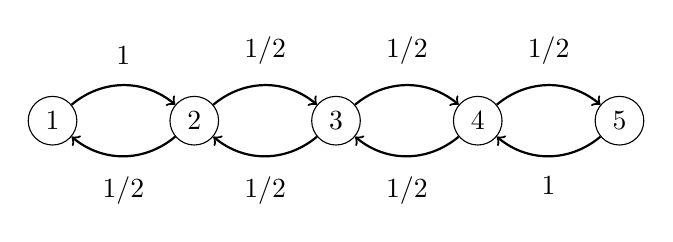
\begin{tikzpicture}[scale=0.9]
\node[draw, circle] (1) at (0,0) {$1$};
\node[draw, circle] (2) at (2,0) {$2$};
\node[draw, circle] (3) at (4,0) {$3$};
\node[draw, circle] (4) at (6,0) {$4$};
\node[draw, circle] (5) at (8,0) {$5$};

\path[draw,thick,->] (1) edge [bend left=40] node[font=\small,label=$1$] {} (2);
\path[draw,thick,->] (2) edge [bend left=40] node[font=\small,label=$1/2$] {} (3);
\path[draw,thick,->] (3) edge [bend left=40] node[font=\small,label=$1/2$] {} (4);
\path[draw,thick,->] (4) edge [bend left=40] node[font=\small,label=$1/2$] {} (5);

\path[draw,thick,->] (5) edge [bend left=40] node[font=\small,label=below:$1$] {} (4);
\path[draw,thick,->] (4) edge [bend left=40] node[font=\small,label=below:$1/2$] {} (3);
\path[draw,thick,->] (3) edge [bend left=40] node[font=\small,label=below:$1/2$] {} (2);
\path[draw,thick,->] (2) edge [bend left=40] node[font=\small,label=below:$1/2$] {} (1);

%\path[draw,thick,->] (1) edge [bend left=40] node[font=\small,label=below:$1$] {} (2);
\end{tikzpicture}
\end{center}

The probability distribution
of a Markov chain is a vector
$[p_1,p_2,\ldots,p_n]$, where $p_k$ is the
probability that the current state is $k$.
The formula $p_1+p_2+\cdots+p_n=1$ always holds.

In the above scenario, the initial distribution is
$[1,0,0,0,0]$, because we always begin in floor 1.
The next distribution is $[0,1,0,0,0]$,
because we can only move from floor 1 to floor 2.
After this, we can either move one floor up
or one floor down, so the next distribution is
$[1/2,0,1/2,0,0]$, and so on.

An efficient way to simulate the walk in
a Markov chain is to use dynamic programming.
The idea is to maintain the probability distribution,
and at each step go through all possibilities
how we can move.
Using this method, we can simulate
a walk of $m$ steps in $O(n^2 m)$ time.

The transitions of a Markov chain can also be
represented as a matrix that updates the
probability distribution.
In the above scenario, the matrix is

\[
 \begin{bmatrix}
  0 & 1/2 & 0 & 0 & 0 \\
  1 & 0 & 1/2 & 0 & 0 \\
  0 & 1/2 & 0 & 1/2 & 0 \\
  0 & 0 & 1/2 & 0 & 1 \\
  0 & 0 & 0 & 1/2 & 0 \\
 \end{bmatrix}.
\]

When we multiply a probability distribution by this matrix,
we get the new distribution after moving one step.
For example, we can move from the distribution
$[1,0,0,0,0]$ to the distribution
$[0,1,0,0,0]$ as follows:

\[
 \begin{bmatrix}
  0 & 1/2 & 0 & 0 & 0 \\
  1 & 0 & 1/2 & 0 & 0 \\
  0 & 1/2 & 0 & 1/2 & 0 \\
  0 & 0 & 1/2 & 0 & 1 \\
  0 & 0 & 0 & 1/2 & 0 \\
 \end{bmatrix}
 \begin{bmatrix}
  1 \\
  0 \\
  0 \\
  0 \\
  0 \\
 \end{bmatrix}
=
 \begin{bmatrix}
  0 \\
  1 \\
  0 \\
  0 \\
  0 \\
 \end{bmatrix}.
\]

By calculating matrix powers efficiently,
we can calculate the distribution after $m$ steps
in $O(n^3 \log m)$ time.

\section{乱択}

\index{乱択}

問題を解くために確率とは関係ない問題だとしても、ランダム性を利用することがあります。
\key{乱択}はランダム性を用いたアルゴリズムです。

\index{モンテカルロ法(Monte Carlo algorithm)}

A \key{モンテカルロ法(Monte Carlo algorithm)} は、
間違った答えとなる可能性を十分に持つランダム化アルゴリズムのことです。
このアルゴリズムが適切であるためには、間違った答えが出る確率が十分に小さいことが必要です。

\index{ラスベガス法(Las Vegas algorithm)}

\key{ラスベガス法}は、間違った答えを出さないが、実行時間はランダムに変化するアルゴリズムである。
このアルゴリズムのデザインには効率的なアルゴリズムの設計が必要です。

次に、ランダム性を利用して解くことができる3つの例題を紹介します。

\subsubsection{k番目に小さい数(Order statistics)}

\index{k番目に小さい数(Order statistics)}

配列の\key{k番目に小さい数(Order statistics)}は
昇順にソートした後の位置kにある要素です。
ですが、ある1つの要素を見つけるためだけに配列全体をソートする必要があるのでしょうか?
実は,配列をソートせずにランダムなアルゴリズムでこれを求めることができます.
これは\key{quickselect}\footnote{In 1961,
C. A. R. Hoare published two algorithms that
are efficient on average: \index{quicksort} \index{quickselect}
\key{quicksort} \cite{hoa61a} for sorting arrays and
\key{quickselect} \cite{hoa61b} for finding order statistics.}
アルゴリズム、別名ラスベガス・アルゴリズムと呼ばれ、その実行時間は通常$O(n)$、最悪の場合$O(n^2)$です。

このアルゴリズムは,配列のランダムな要素$x$を選んで,$x$より小さい要素を配列の左に,
それ以外の要素を配列の右側に移動させます.
これは要素がn個のとすると,O(n)で実行できます。
左側には $a$ 個の要素,右側には $b$ 個の要素があるとしましょう。
さて、$a = k$ ならば,要素 $x$ はk番目に小さい数です。
$a > k$ の時は左側部分の $k$番目の数を再帰的に求め,
$a < k$ の時は右側部分の $r$ 番目の数$(r = k - a)$を再帰的に求め,
要素が見つかるまで同様の方法で探索を見つければ良いのです。


$x$ がランダムに選ばれるため,配列のサイズは各ステップで約半分と期待できるので,この時間計算量は次のようになります。
\[n+n/2+n/4+n/8+\cdots < 2n = O(n).\]

最悪の場合は$O(n^2)$です。
これは$x$ が配列の最小または最大の要素の1つになるように常に選択される場合で$O(n)$ ステップが必要になるからです.
しかし、その確率は非常に小さいので、実際にはこのようなことは起こらないでしょう。

\subsubsection{Verifying matrix multiplication}

\index{matrix multiplication}

Our next problem is to \emph{verify}
if $AB=C$ holds when $A$, $B$ and $C$
are matrices of size $n \times n$.
Of course, we can solve the problem
by calculating the product $AB$ again
(in $O(n^3)$ time using the basic algorithm),
but one could hope that verifying the
answer would by easier than to calculate it from scratch.

It turns out that we can solve the problem
using a Monte Carlo algorithm\footnote{R. M. Freivalds published
this algorithm in 1977 \cite{fre77}, and it is sometimes
called \index{Freivalds' algoritm} \key{Freivalds' algorithm}.} whose
time complexity is only $O(n^2)$.
The idea is simple: we choose a random vector
$X$ of $n$ elements, and calculate the matrices
$ABX$ and $CX$. If $ABX=CX$, we report that $AB=C$,
and otherwise we report that $AB \neq C$.

The time complexity of the algorithm is
$O(n^2)$, because we can calculate the matrices
$ABX$ and $CX$ in $O(n^2)$ time.
We can calculate the matrix $ABX$ efficiently
by using the representation $A(BX)$, so only two
multiplications of $n \times n$ and $n \times 1$
size matrices are needed.

The drawback of the algorithm is
that there is a small chance that the algorithm
makes a mistake when it reports that $AB=C$.
For example,
\[
 \begin{bmatrix}
  6 & 8 \\
  1 & 3 \\
 \end{bmatrix}
\neq
 \begin{bmatrix}
  8 & 7 \\
  3 & 2 \\
 \end{bmatrix},
\]
but
\[
 \begin{bmatrix}
  6 & 8 \\
  1 & 3 \\
 \end{bmatrix}
 \begin{bmatrix}
  3 \\
  6 \\
 \end{bmatrix}
=
 \begin{bmatrix}
  8 & 7 \\
  3 & 2 \\
 \end{bmatrix}
 \begin{bmatrix}
  3 \\
  6 \\
 \end{bmatrix}.
\]
However, in practice, the probability that the
algorithm makes a mistake is small,
and we can decrease the probability by
verifying the result using multiple random vectors $X$
before reporting that $AB=C$.

\subsubsection{Graph coloring}

\index{coloring}

Given a graph that contains $n$ nodes and $m$ edges,
our task is to find a way to color the nodes
of the graph using two colors so that
for at least $m/2$ edges, the endpoints
have different colors.
For example, in the graph
\begin{center}
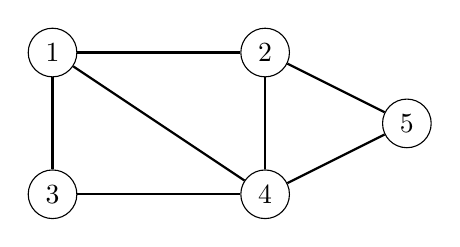
\begin{tikzpicture}[scale=0.9]
\node[draw, circle] (1) at (1,3) {$1$};
\node[draw, circle] (2) at (4,3) {$2$};
\node[draw, circle] (3) at (1,1) {$3$};
\node[draw, circle] (4) at (4,1) {$4$};
\node[draw, circle] (5) at (6,2) {$5$};

\path[draw,thick,-] (1) -- (2);
\path[draw,thick,-] (1) -- (3);
\path[draw,thick,-] (1) -- (4);
\path[draw,thick,-] (3) -- (4);
\path[draw,thick,-] (2) -- (4);
\path[draw,thick,-] (2) -- (5);
\path[draw,thick,-] (4) -- (5);
\end{tikzpicture}
\end{center}
a valid coloring is as follows:
\begin{center}
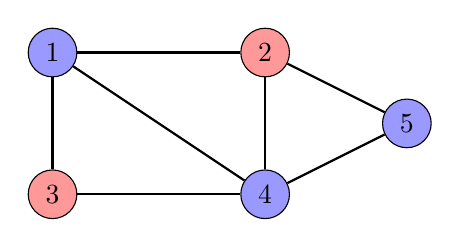
\begin{tikzpicture}[scale=0.9]
\node[draw, circle, fill=blue!40] (1) at (1,3) {$1$};
\node[draw, circle, fill=red!40] (2) at (4,3) {$2$};
\node[draw, circle, fill=red!40] (3) at (1,1) {$3$};
\node[draw, circle, fill=blue!40] (4) at (4,1) {$4$};
\node[draw, circle, fill=blue!40] (5) at (6,2) {$5$};

\path[draw,thick,-] (1) -- (2);
\path[draw,thick,-] (1) -- (3);
\path[draw,thick,-] (1) -- (4);
\path[draw,thick,-] (3) -- (4);
\path[draw,thick,-] (2) -- (4);
\path[draw,thick,-] (2) -- (5);
\path[draw,thick,-] (4) -- (5);
\end{tikzpicture}
\end{center}
The above graph contains 7 edges, and for 5 of them,
the endpoints have different colors,
so the coloring is valid.

The problem can be solved using a Las Vegas algorithm
that generates random colorings until a valid coloring
has been found.
In a random coloring, the color of each node is
independently chosen so that the probability of
both colors is $1/2$.

In a random coloring, the probability that the endpoints
of a single edge have different colors is $1/2$.
Hence, the expected number of edges whose endpoints
have different colors is $m/2$.
Since it is expected that a random coloring is valid,
we will quickly find a valid coloring in practice.
